% 
% Annual Cognitive Science Conference
% Sample LaTeX Paper -- Proceedings Format
% 

% Original : Ashwin Ram (ashwin@cc.gatech.edu)       04/01/1994
% Modified : Johanna Moore (jmoore@cs.pitt.edu)      03/17/1995
% Modified : David Noelle (noelle@ucsd.edu)          03/15/1996
% Modified : Pat Langley (langley@cs.stanford.edu)   01/26/1997
% Latex2e corrections by Ramin Charles Nakisa        01/28/1997 
% Modified : Tina Eliassi-Rad (eliassi@cs.wisc.edu)  01/31/1998
% Modified : Trisha Yannuzzi (trisha@ircs.upenn.edu) 12/28/1999 (in process)
% Modified : Mary Ellen Foster (M.E.Foster@ed.ac.uk) 12/11/2000
% Modified : Ken Forbus                              01/23/2004
% Modified : Eli M. Silk (esilk@pitt.edu)            05/24/2005
% Modified : Niels Taatgen (taatgen@cmu.edu)         10/24/2006
% Modified : David Noelle (dnoelle@ucmerced.edu)     11/19/2014

%% Change "letterpaper" in the following line to "a4paper" if you must.

\documentclass[10pt,letterpaper]{article}

\usepackage{cogsci}
\usepackage{pslatex}
\usepackage{apacite}

\usepackage{tikz}
\usetikzlibrary{arrows,shapes,snakes,automata,backgrounds,petri}

\title{Curiosity-Driven Development of Tool Use Precursors: a Robotic Model}
 
\author{{\large \bf S\'ebastien Forestier (sebastien.forestier@inria.fr)} \\
	INRIA Bordeaux Sud-Ouest\\
	Bordeaux, France
  \AND {\large \bf Pierre-Yves Oudeyer (pierre-yves.oudeyer@inria.fr)} \\
	INRIA Bordeaux Sud-Ouest\\
	Bordeaux, France}

\usepackage[caption=false,font=footnotesize]{subfig}


\begin{document}

\maketitle


\begin{abstract}
This is the abstract.

\textbf{Keywords:} 
curiosity-driven learning; tool use; goal babbling; overlapping waves; 
\end{abstract}


\section{Introduction}

	Development of tool use \cite{guerin2013survey}, precursors of tool use: behavior without objects, behavior with one object, interaction of objects.	
	Grounding of representation and planning based on a large amount of experiences. 	
	Seemless progression between the successives phases as overlapping waves. 	
	Ongoing process of upgrading representations.	
	Developmental trajectories.
	
	
	Curiosity studies in developmental psychology 
	\cite{kidd}
	\cite{gottlieb_information-seeking_2013}
	
	Curiosity-driven modelling work, emergence of developmental trajectories.
	\cite{oudeyer_intrinsic_2007} 
	\cite{oudeyer_what_2007}
	\cite{flow}
	\cite{sch}
	\cite{santucci2013}
	\cite{cangelosi2010integration}
	\cite{oudeyer2014evolution}
	
	
	IAC series of architectures and Explauto framework: previous experiments.
	\cite{moulin-frier_self-organization_2014}
	\cite{moulin-frier_explauto:_2014}
	\cite{baranes2010intrinsically}
	\cite{riac}
	\cite{baranes_active_2013}
	
	Representations in explauto and other models 
	\cite{mugan2009}
	\cite{metzen2013}
	\cite{horde}
	\cite{mugan}
	\cite{vig}
	\cite{sutton1999between}
	
	Other related work
	\cite{ugur2015}
	\cite{schmerlinggoal}

	More details on experiments
	\cite{ijspeert_dynamical_2013}
	
	\cite{}
	
%

\section{Methods}

	\subsection{Environment}
	
		\paragraph{}
		We simulate a 2D robotic arm using tools to move an object into different boxes in the environment. 		
		In each trial, we execute a motor trajectory given by the agent, we evaluate its consequences on the sensory dimensions and we give him
		this sensory feedback. Finally the arm, tools and objects are resetted to their intial state.
		
		The next sections precisely describe the different items of the environment and their interactions.	
		See Fig.\ref{env} for an exemple of the state of the environment. 
		
		\begin{figure}[h]
			\centering
			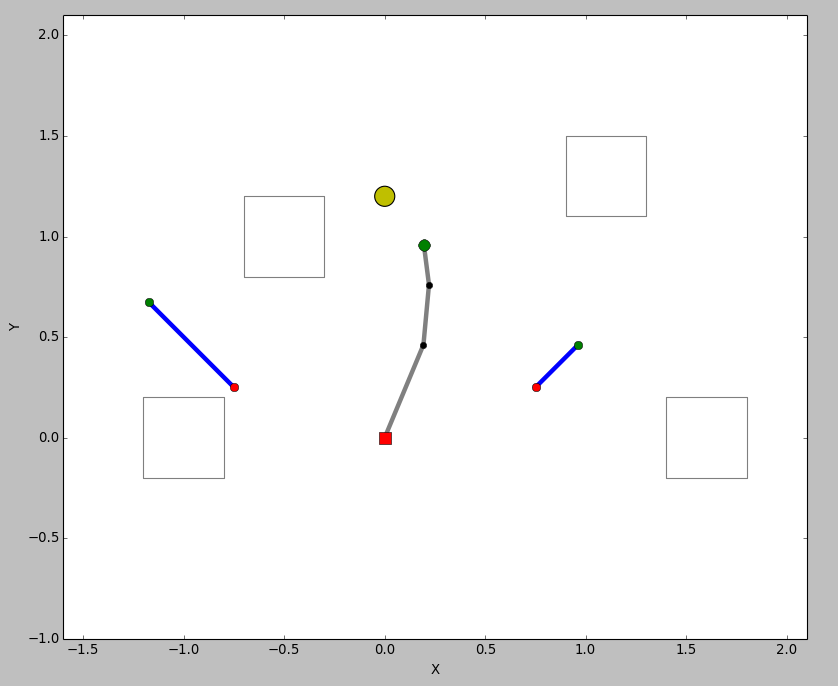
\includegraphics[width=8cm]{./include/tools.png}
			\caption{Play Environment}
			\label{env}
		\end{figure}
			

		\subsubsection{Robotic arm}
		
			The 2D robotic arm has 3 joints plus a gripper located at the end-effector.
			Each joint can rotate from $-\pi~rad$ to $\pi~rad$ around its initial position, mapped to a standard interval of $[-1,1]$.
			The length of the 3 parts of the arm are $0.5$, $0.3$ and $0.2$ so the total length of the arm is $1$ unit.
			The initial position of the arm is vertical with each joint at $0~rad$ and its base is fixed at position $[0, 0]$.
			The gripper $g$ has 2 possible positions: \textit{open} ($g \geq 0$) and \textit{closed} ($g < 0$) and its initial position is \textit{open} (with $g = 0$).
			The robotic arm thus has 4 degrees of freedom represented by a vector in $[-1,1]^4$.
			A trajectory of the arm will be represented as a sequence of such vectors.\\
		
		%
		
		\subsubsection{Motor control}
		
			We use Dynamical Movement Primitive \cite{ijspeert_dynamical_2013} to control the arm's movement as this framework permits the production of a diversity of arm's trajectories with few parameters.
			Each of the $4$ arm's degrees-of-freedom (DOF) is controlled by a DMP with a starting and a goal position equal to the rest position of the joint.
			Each DMP is parameterized by one weight on each of $3$ basis functions whose centers are distributed homogeneously throughout the movement duration.
			The weights are bounded in the interval $[-200,200]$ (mapped to the standard interval $[-1,1]$) which allow each joint to fairly cover the interval $[-1,1]$ during the movement.
			Each DMP outputs a series of $50$ positions that represents a sampling of the trajectory of one joint during the movement.		
			The arm's movement is thus parameterized by $12$ weights which are represented by the motor space $M=[-1,1]^{12}$.\\
		
		%
			
		\subsubsection{Objects and tools}
			
			A yellow sphere can be moved into one of the 4 fixed squared boxes. 
			The initial position of the sphere is $(0, 1.2)$ and is thus unreachable directly with the gripper.
			One of two sticks can be grasped in order to reach the object.
			A small stick of length $0.3$ is located on the right of the arm, with initial position $(0.75, 0.25)$ and initial angle $\frac{\pi}{4}$ from the horizontal line.
			A long stick of length $0.6$ is located on the left of the arm, with initial position $(-0.75, 0.25)$ and initial angle $\frac{3\pi}{4}$ from the horizontal line as in Fig. \ref{env}.			
			If the gripper closes near the end of one of the sticks (closer than $0.1$), it is considered grasped and will follow the gripper's position and the angle of the arm's last part until the gripper opens.			
			Similarly, if the other end of a stick reaches the sphere (within $0.1$), the object will follow the end of the stick.
			Ten boxes have identifiers $1$ to $10$ and are static at positions $(-1.4, 0)$, $(-1.1, 1.1)$, $(0, 1.4)$, $(1.1, 1.1)$, $(1.4, 0)$, $(-0.9, 0)$, $(-0.6, 0.6)$, $(0, 0.9)$, $(0.6, 0.6)$ and $(0.9, 0)$ and have size $0.2$.
			The first five boxes can only be reached with the long stick, and the other five can be reached by the two sticks.
			At the end of the trial, the object is considered to be in one of the box if its center is in the box.\\
		
		%
		
		\subsubsection{Sensory feedback}
		
			At the end of the movement, the robot gets sensory feedback from the different items of the environment.
			It gets the trajectory of its hand and gripper, the trajectory of the end of the sticks, 
			the end position of the object, and whether the object is in each box.		
			The trajectory of the hand and of the end point of the sticks are represented by sequences of x and y positions at different time points: 
			steps $12$, $25$, $37$ during the movement of $50$ steps ($6$D for the hand and for each stick).
			Similarly, the trajectory of the gripper is a sequence of $1$ or $-1$ depending whether the gripper is open or closed ($3$D).
			The agent receives the identifier of the reached box if one of them has been reached, 0 otherwise. He also gets the minimal distance of the object (at the end of the movement) to the center a box, even if none have been reached.
			%For each box, the robot receives a $1$ if the object is in the box at the end of the movement, and $0$ otherwise ($4$D).			 
			The sensory information thus contains $9$ values for the trajectory of the hand and gripper ($S_{Hand}$), $6$ for the trajectory of the end of each stick ($S_{Stick_1}$ and $S_{Stick_2}$), $2$ for the end position of the object ($S_{Object}$) and $2$ for the boxes ($S_{Boxes}$).
			The sensory space has a total of $25$ dimensions.
			
		%
		
	%
	
	\subsection{Learning architectures}

		We describe in this section the different learning architectures used in the experiment. 
		
		\subsubsection{Explauto framework}
			
			We use the Explauto autonomous exploration library \cite{moulin-frier_explauto:_2014} to easily define experiments with robots exploring their environment. 
			In this framework, the agent explores a mapping between its given motor space $M$ and sensory space $S$, 
			using a sensorimotor model that learns the mapping and an interest model that chooses which regions of the spaces to explore.
			The sensorimotor model processes new information of the form ($m, s$) with $m \in M$ being the experimented motor parameters and $s \in S$ the received sensory feedback 
			corresponding to that parameters. 
			It provides forward predictions of probable $s$ given $m$ and inverse inference of a probable $m$ to reach a given $s$.
			We use the simplest sensorimotor model, the nearest neighbor algorithm 
			that performs the prediction of $s$ given $m$ using the nearest neighbor of $m$ in $M$ in the database of the previous experiments and returning its sensory part. 
			The inverse inference is computed as the motor part of the nearest neighbor in $S$ of the given $s$, but with some exploration noise to allow novel motor parameters to be explored.
			
			The agent also needs an interest model that chooses which regions of the motor or sensory space to explore.
			If the agent chooses goals in the motor space and explores them it is called Motor Babbling, and if it chooses the goals to explore in the sensory space, this is Goal Babbling.
			To choose the goals in this space of interest, different strategies are possible. 
			The simplest one is to draw random goals in this space, but strategies based on the learning progress in different regions of the space have been shown more efficient in [ref].
			This strategies are called active as the agent autonomously drives its exploration towards regions of the space that are both reachable and learnable. 
			We use the SAGG-RIAC architecture \cite{baranes_active_2013} where the space of interest is the sensory space (Goal Babbling) and that incrementally splits this space into subregions where the learning progress 
			is different.
			
				
		%
		
		\subsubsection{Flat architecture}
			
				
		%
		
		\subsubsection{Hierarchical architecture}
			
			We present here an architecture that represents sensorimotor information with a hierarchical structure in Fig. \ref{H1}.
			
			Only the motor module (mod1) adds exploration noise ($\sigma=0.02$) even in hierarchical architecture. 
			That was the key to have more efficient hierarchical exploration. 
			Indeed, if all modules successively add exploration noise, few iterations succeed in touching the object. 
			Alternatively, if the exploration noise is reduced, exploration is less efficient as in NN only the motor module will finally apply noise on known motor commands. 
			With regression instead of NN, noise can instead be put only on the babbling module.
			
			How competence and interest of modules is computed.
			
			\begin{figure}[t]
				\center
				
% H2
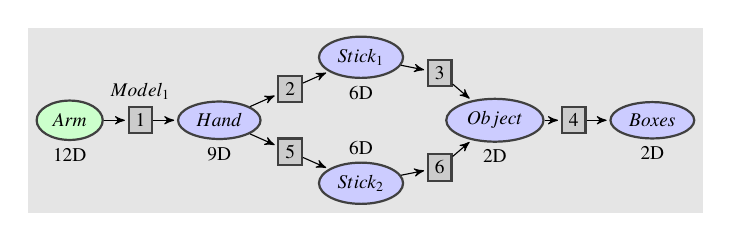
\begin{tikzpicture}[node distance=1cm,>=stealth',bend angle=45,auto]

	\tikzstyle{dom}   = [ellipse, thick, draw=black!75, fill=blue!20,  minimum height=4mm, minimum width=4mm]
	\tikzstyle{prim dom}   = [dom,  minimum height=5mm, minimum width=5mm,  fill=green!20]
	\tikzstyle{mod} = [rectangle, thick, draw=black!75, fill=black!20, minimum size=3mm]

	\begin{scope}
		\scriptsize
		\node [prim dom, label=below:$12$D] (pd1) {$Arm$};

		\node [mod, label=above:$Model_1$] (m1) [right of=pd1, xshift=-0.1cm] {$1$}
		edge [pre]                  (pd1);

		\node [dom, label=below:$9$D] (d1) [right of=m1] {$Hand$}
		edge [pre]                (m1);
		
		\node [mod] (m3) [right of=d1, xshift=-0.1cm,yshift=0.4cm] {$2$}
		edge [pre]                  (d1);
		
		\node [dom, label=below:$6$D] (d3) [right of=m3, xshift=-0.1cm,yshift=0.4cm] {$Stick_1$}
		edge [pre]                (m3);
		
		\node [mod] (m6) [right of=d1, xshift=-0.1cm,yshift=-0.4cm] {$5$}
		edge [pre]                  (d1);
		
		\node [dom, label=above:$6$D] (d6) [right of=m6, xshift=-0.1cm,yshift=-0.4cm] {$Stick_2$}
		edge [pre]                (m6);
		
		\node [mod] (m7) [right of=d6,yshift=0.2cm] {$6$}
		edge [pre]                  (d6);
		
		\node [mod] (m4) [right of=d3,yshift=-0.2cm] {$3$}
		edge [pre]                  (d3);
		
		\node [dom, label=below:$2$D] (d4) [right of=m4, xshift=-0.3cm,yshift=-0.6cm] {$Object$}
		edge [pre]                (m4)
		edge [pre]                (m7);
		
		\node [mod] (m5) [right of=d4] {$4$}
		edge [pre]                  (d4);
		
		\node [dom, label=below:$2$D] (d5) [right of=m5] {$Boxes$}
		edge [pre]                (m5);
		
		
	\end{scope}
	\begin{pgfonlayer}{background}
		\filldraw [line width=2mm,black!10]
		(d3.north  -| d5.east)  rectangle (d6.south  -| pd1.west);
	\end{pgfonlayer}
\end{tikzpicture}

				\caption{Hierarchy of sensorimotor models}
				\label{H1}					
			\end{figure}

				
		%
		

	%
	
	\subsection{Experiments}
		
		NN, $100$ iterations of Motor babbling and then $300000$ iterations of the condition. 10 trials per condition, mean and std provided.
		
		
		\subsubsection{Conditions}
			
			\begin{itemize}
			
				\item H0-MB: Random Motor Babbling
				\item H0-GB: Random Goal Babbling with a flat architecture learning $$M \rightarrow S_{Hand} \times S_{Stick_1} \times S_{Stick_2} \times S_{Object} \times S_{Boxes}$$
				\item H0-TR: The same architecture but with active goal babbling (my version of SAGG-RIAC)
				\item H1: Hierarchical architecture with Random Goal Babbling in each module, and choice of module that babbles based on interest ($\epsilon$-prop: probabilities proportional to interest but with $\epsilon=10\%$ of random choice). Choice of tool to use based on the maximum interest of the two modules that learn from the spaces of the tools to the object space, around the goal object point (competence progress on the k=10 NN).
				\item H1-GR: same as H1 but the choice of module to babble is $\epsilon$-greedy with $\epsilon=0.1$
				\item H1-CL: same as H1 but the choice of the tool to use is based on the maximum competence around the goal object point (competence of the NN)
			
			\end{itemize}
				
		%
		
		\subsubsection{Measures}
			
			Exploration of the different sensory spaces (number of reached cells in a discretization of the space divided by number of cells).
			
		%
		
	%
	
%


\section{Results}
	
	\paragraph{}
	We measure the exploration of the different sensory spaces in the $6$ conditions each $5000$ iterations along the $300000$ iterations (Fig. \ref{res_explo}).
	We provide statistical Mann-Whitney U test results of comparisons of the exploration at the end of the experiments in different pairs of conditions.
	We first show that the Motor Babbling condition (H0-MB) quickly explores $S_{Hand}$ but explores badly the other sensory spaces, compared to the other conditions (STATS).
	Then H0-GB and H0-Tr have similar exploration results (STATS maybe Tr better in Boxes).
	Then H1-GR shows lower exploration of $S_{Hand}$, $S_{Stick_1}$ and $S_{Stick_2}$ than H0-GB and H0-Tr but higher exploration of $S_{Object}$ and $S_{Boxes}$ (STATS).
	Also, H1-GR shows lower exploration of all spaces than H1 (STATS).
	H1 shows lower exploration of $S_{Hand}$ than H0-GB and H0-Tr (STATS), similar (STATS?) exploration of $S_{Stick_1}$ and $S_{Stick_2}$ but higher exploration of $S_{Object}$ and $S_{Boxes}$ (STATS).
	H1-CL vs H1 (STATS?).
	
	\begin{figure*}[ht]
		\centering
		\subfloat[$Hand$]{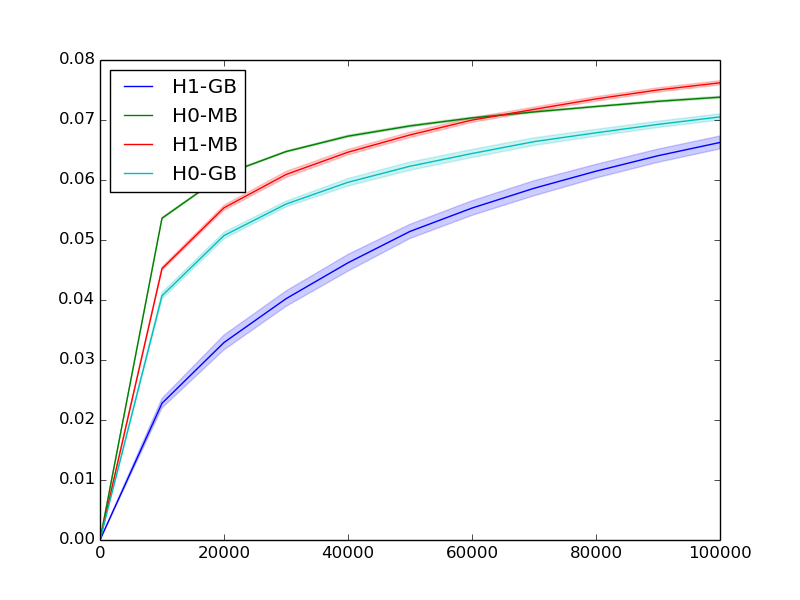
\includegraphics[width=4.5cm]{./include/xp1-explo-hand.png}}
		\subfloat[$Stick_1$]{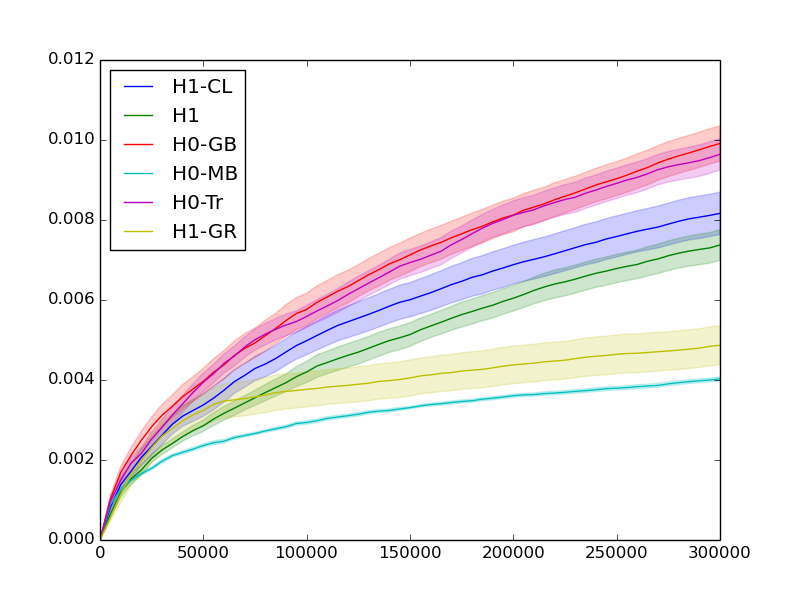
\includegraphics[width=4.5cm]{./include/xp1-explo-stick_1.png}}
		\subfloat[$Stick_2$]{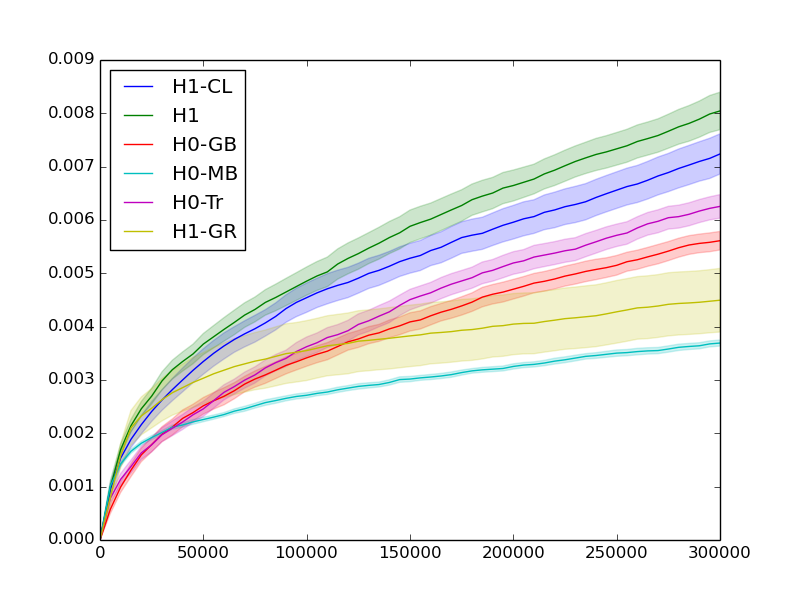
\includegraphics[width=4.5cm]{./include/xp1-explo-stick_2.png}}\\
		\subfloat[$Object$]{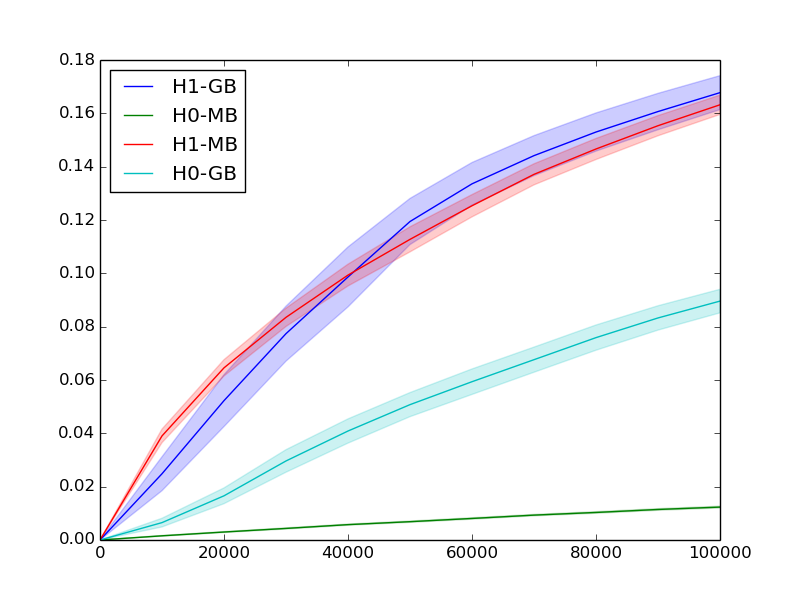
\includegraphics[width=4.5cm]{./include/xp1-explo-obj.png}}
		\subfloat[$Boxes$]{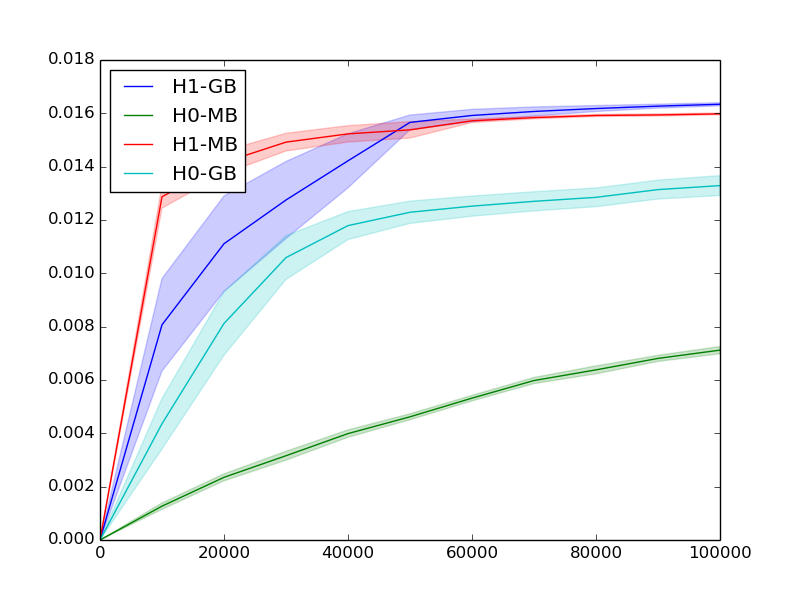
\includegraphics[width=4.5cm]{./include/xp1-explo-box.png}}
		\caption{Exploration of sensory spaces.}
		\label{res_explo}
	\end{figure*}


	\paragraph{}
	Fig. \ref{res_interests} shows more details about one (randomly chosen) trial of the condition H1. 
	We can see the interest of each module during the whole experiment.
	The interests of modules 1, 2, 5 are almost stable, as the spaces of interests are high-dimensional and homogeneously reachable: a random exploration will find regions to learn more for more iterations than $300000$.
	The interests of modules 3 and 6 increase abruptly when the object is touch by the corresponding tool.
	An exemple of exploration of the $2$D space with the object is also provided in Fig. \ref{res_interests}(b) also corresponding to condition H1.
	
	\begin{figure*}[ht]
		\subfloat[]{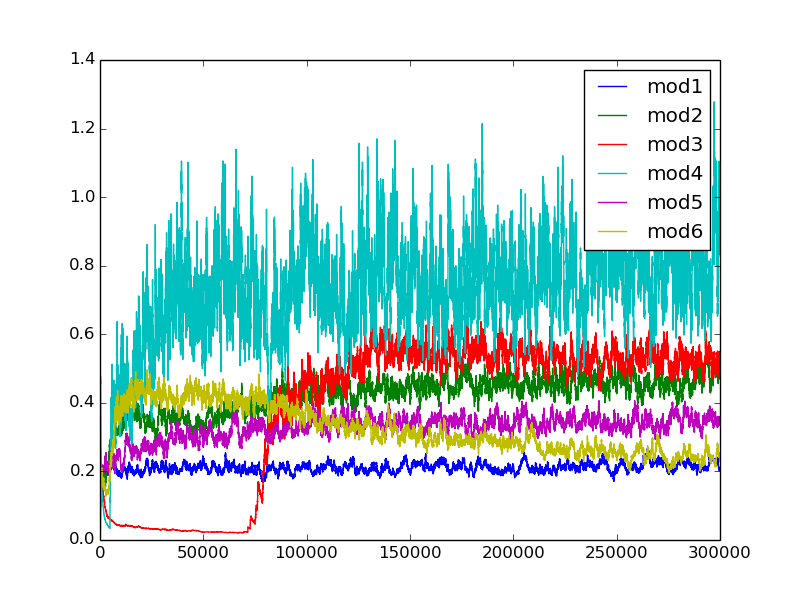
\includegraphics[width=9cm]{./include/H1-log3-interests.png}}
		\subfloat[]{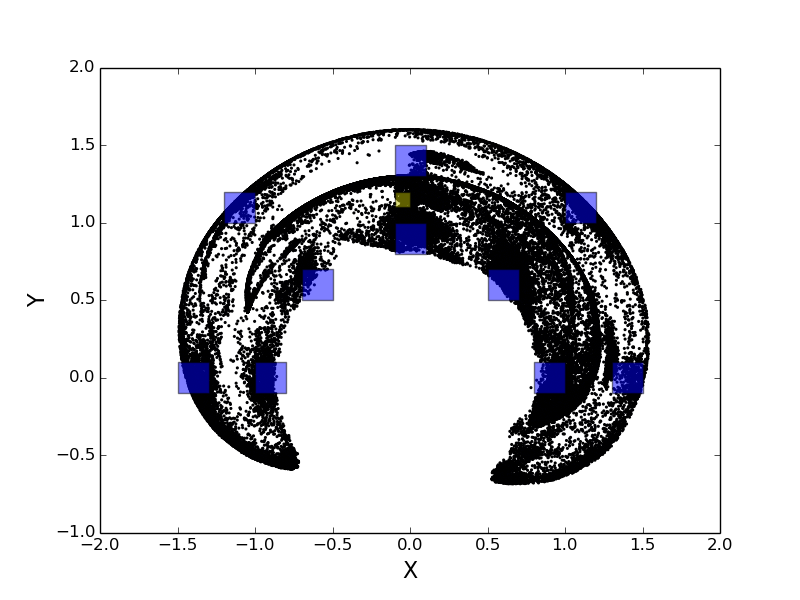
\includegraphics[width=9cm]{./include/H1-log3-obj-explo.png}}
		\caption{Condition H1. (a) Interests of each module. (b) Exploration of the object space: each dot is one point reached with the object at the end of one movement.}
		\label{res_interests}
	\end{figure*}


	\paragraph{}
	Fig. \ref{res_choice} shows a comparison of the choice of tool to reach a given object goal position in the conditions H1 and H1-CL.
	In those conditions, module $4$ learns a mapping between $S_{Object}$ and $S_{Boxes}$. 
	When this module is babbling (give \# babbling in the 2 conditions: around $100000$), it chooses a random goal $s_b \in S_{Boxes}$ and infers the best object position $s_o$ to reach $s_b$.
	To reach $s_o$, one of the tools ($Stick_1$ with module $3$ or $Stick_2$ with module $6$) has to be chosen. 
	We plot all those choices, at position $s_o$ on a $2$D space, with color blue if $Stick_1$ was chosen and red if $Stick_2$ was chosen, with one plot for each of the two conditions.
	We see (or soon will see in new plots, and maybe with smoothed stats along trials?) that in both conditions, 
	goals that can only be reached with the long stick (the furthest) are actually chosen to be explored with the long stick.
	However, goal that can be reached with both tools are more often chosen to be explored with the long stick in the interest-based choice of condition H1 than in competence-based choice of condition H1-CL.
	
	\begin{figure*}[ht]
		\subfloat[H1]{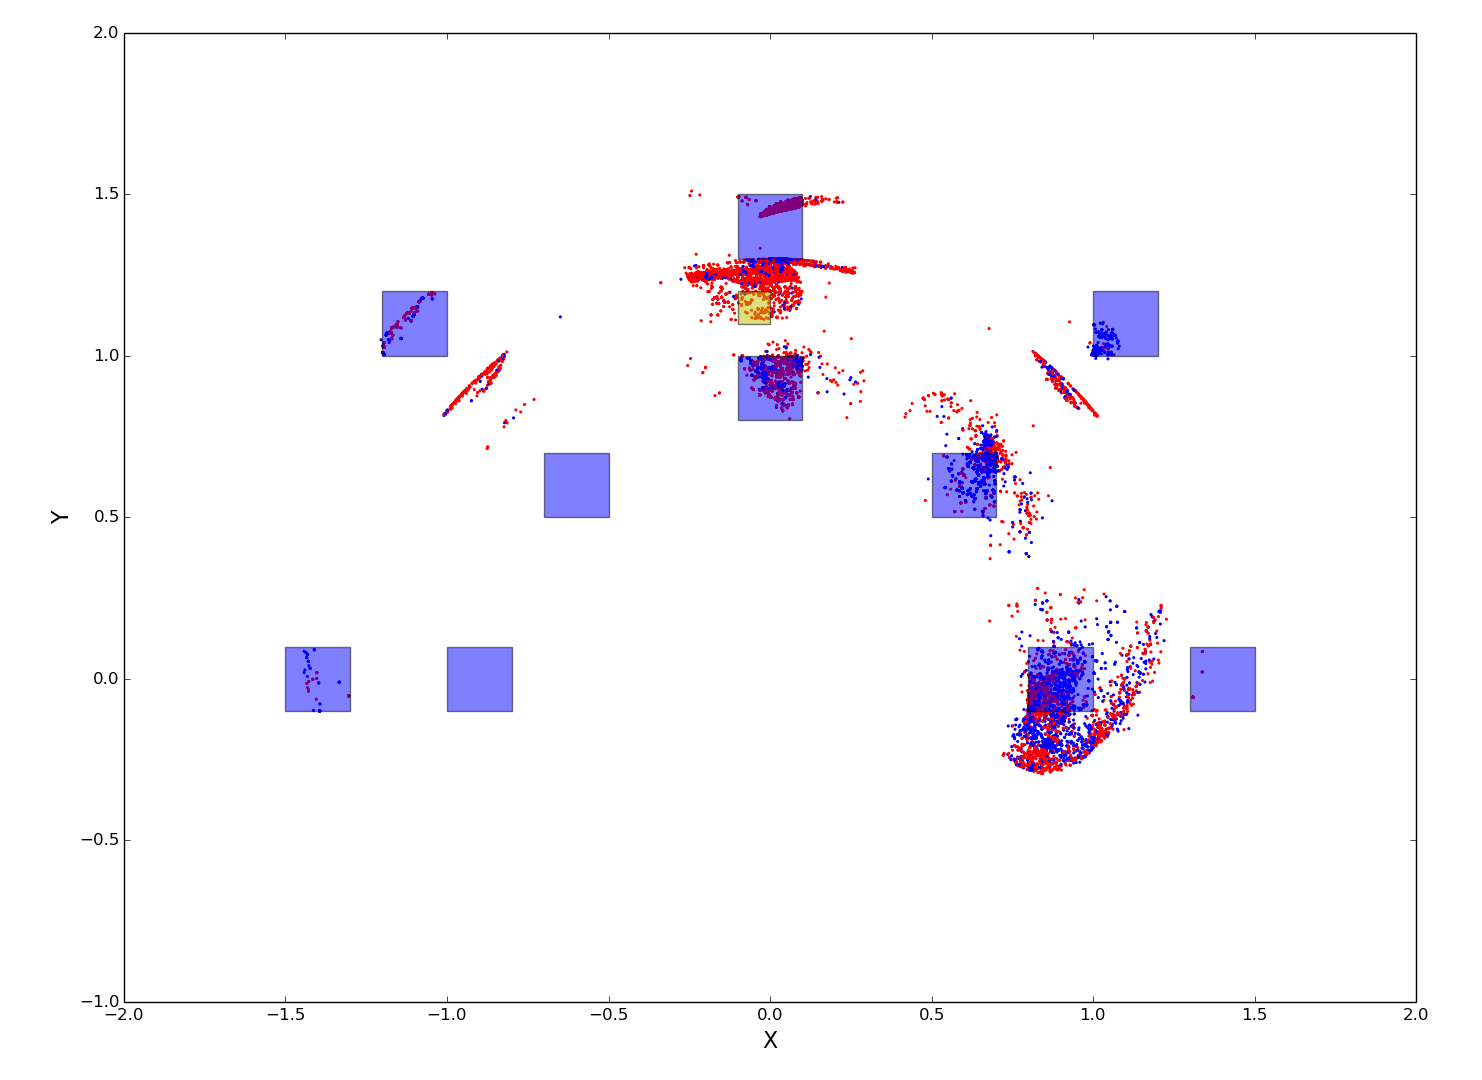
\includegraphics[width=9cm]{./include/choice_mod4_H1.png}}
		\subfloat[H1-CL]{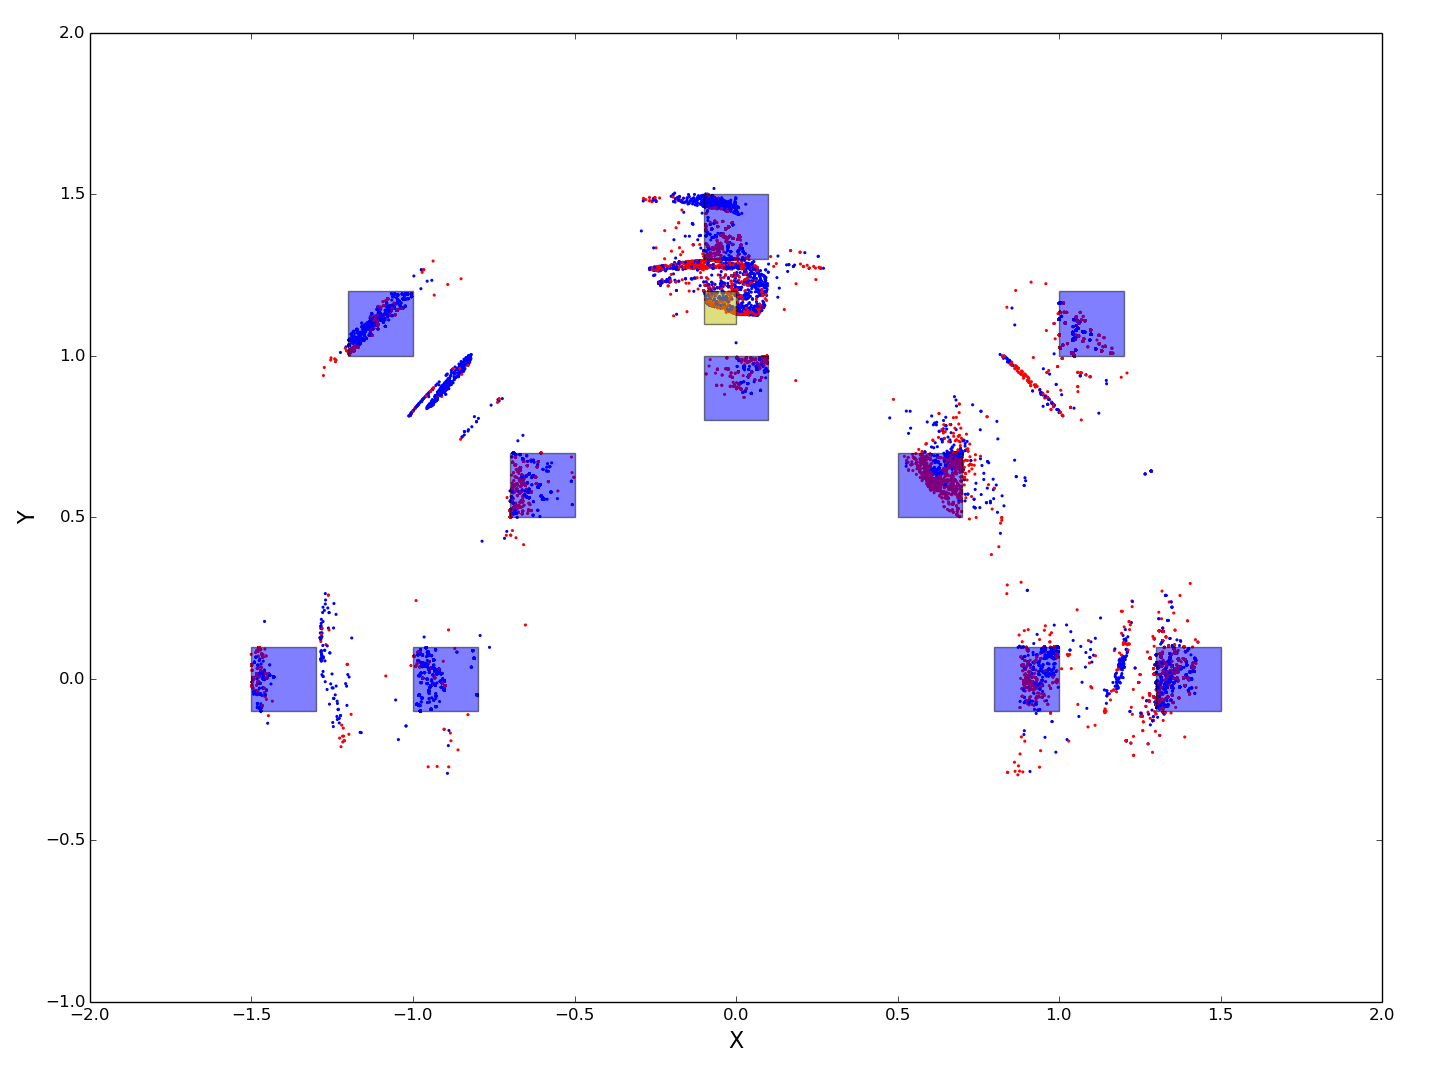
\includegraphics[width=8.8cm]{./include/choice_mod4_H1-CL.png}}
		\caption{Chosen tool depending on object goal position. Blue points: long stick choice. Red points: small stick choice.}
		\label{res_choice}
	\end{figure*}
	
%


\section{Discussion}

	\subsection{H0 vs H1-GR vs H1}
	
	
	%
	
	\subsection{H1 vs H1-CL}
	
	
	%
	
%


\section{Conclusion}

%


\section{Acknowledgments}

%




\bibliographystyle{apacite}

\setlength{\bibleftmargin}{.125in}
\setlength{\bibindent}{-\bibleftmargin}

\bibliography{include/bibliography}


\end{document}
